

%!TEX root = ./main.tex
\chapter{Approach
\label{chapter:approach}}

\section{Methodology
\label{section:methodology}}

To achieve the goal of enhancing the traffic preselection of \gls{FACT} with
knowledge about the past stability and popularity characteristics, the following
three steps are planned for extending \gls{FACT} as illustrated in figure 
\ref{fig:FACT}.

In a first step, a network service detector (server socket detector) is 
implemented. The challenge of the network service detection lies in the fact 
that the flow-level data does not provide enough precise timing information to 
determine which flow is originated from the client and thereof deducing the 
server's socket\citep{Trammell}. Therefore, the network service detection is 
achieved by the assumption that network services offered by servers act as 
concentrators in the sense that several clients have connections to this 
specific service. This approach bases on the work shown in 
\cite{Schatzmann:Dissection, Schatzmann:Mining, Schatzmann:Tracing} and is 
discussed in more detail in section \ref{section:socket_detection}.

\begin{figure}
	[t] \centering
	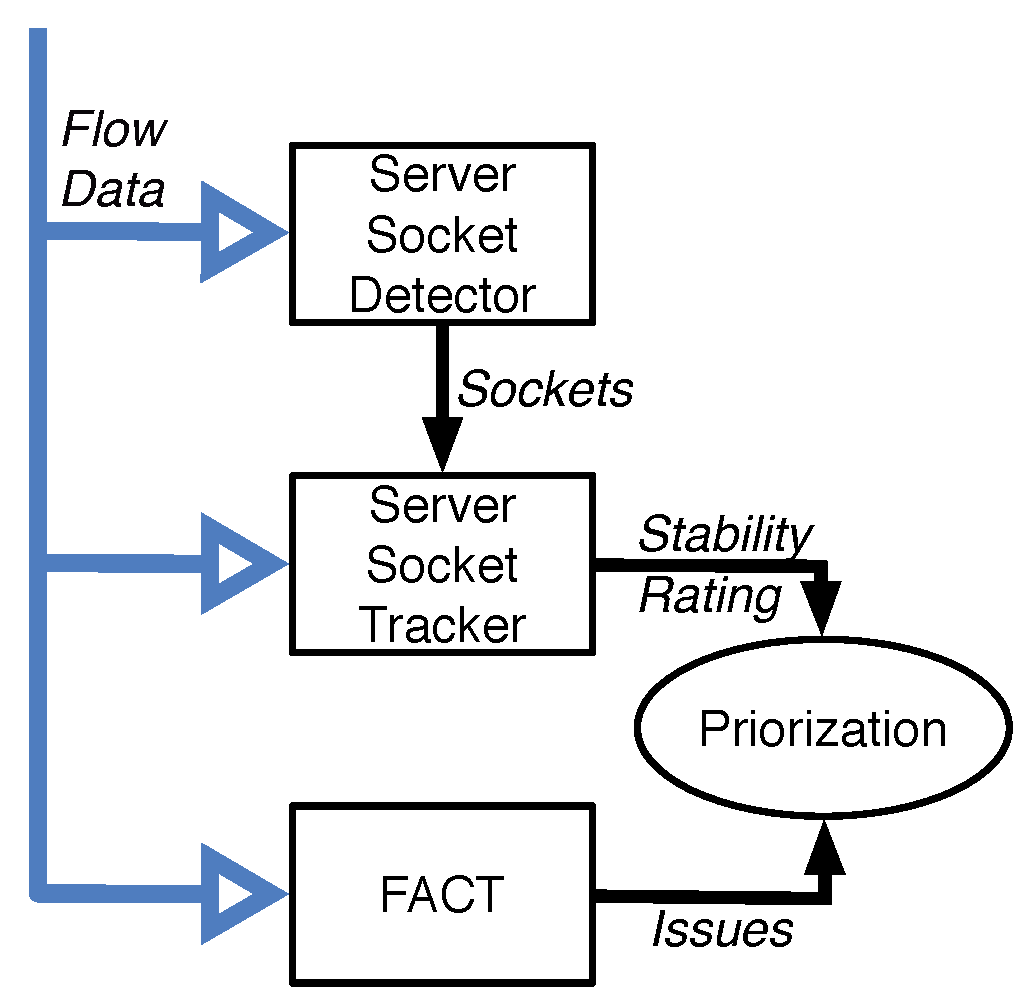
\includegraphics[width=8.5cm]{images/Approach_blockdiagram.eps}
	\caption{Interactions of new components with \gls{FACT}} 
	\label{fig:FACT} 
\end{figure}

Secondly, the previously detected network services are continually monitored and
especially the successful and unsuccessful connection attempts are recorded by
a network service monitoring engine (server socket tracker).
Furthermore, these information are used to statistically characterize the 
network services by their visibility, popularity and stability. Section 
\ref{section:socket_tracking} covers this step in detail.

In a third step, by selecting a set of suitable network services such that 
\gls{FACT} is able to use these sockets for outage tracking. For this reason, 
the number of network services which should be observed by \gls{FACT} have to be 
reduced. To this end, the properties of these observation set has to be 
assessed, because they influences the observation capabilities of \gls{FACT}. 
Particularly, the sets Internet address space coverage is a crucial 
property. With respect to FACTs goal of detecting remote network 
outages, it makes for example no sense to select only the most popular sockets 
if they are all located in the same network. Section \ref{section:ses_selection} 
is discussing this problem in detail. 

Consequently, \gls{FACT} has to be adopted to use the preselected and rated 
network services for prioritizing relevant connectivity issues by reducing 
outage alerts based on single host outages of unstable services. This step is 
further discussed in chapter \ref{chapter:integration}.

%%%%%%%%%%%%%%%%%%%%%%%%%%%%%%%%%%%%%%%%%%%%%%%%%%%%%%%%%%%%%%%%%%%%%%%%%%%%%%%%
\section{Data
\label{section:data}}

This thesis relies on data collected at \citet{switch}, the Swiss National 
Research and Education Network (NREN). Mainly government institutions, 
universities, research labs are connected to the Internet by \citet{switch}\citep{Schatzmann:Mining}.

The \citet{switch} network is with approximately 250'000 network users in 2010 comparable with a mid sized \gls{isp}. Currently, there are around 2.4 million \gls{IPv4} addresses, a /32 IPv6 and a /40 \gls{IPv6} network announced via \gls{bgp}\citep{Schatzmann:Tracing}.

\begin{figure}[b] 
	\centering
	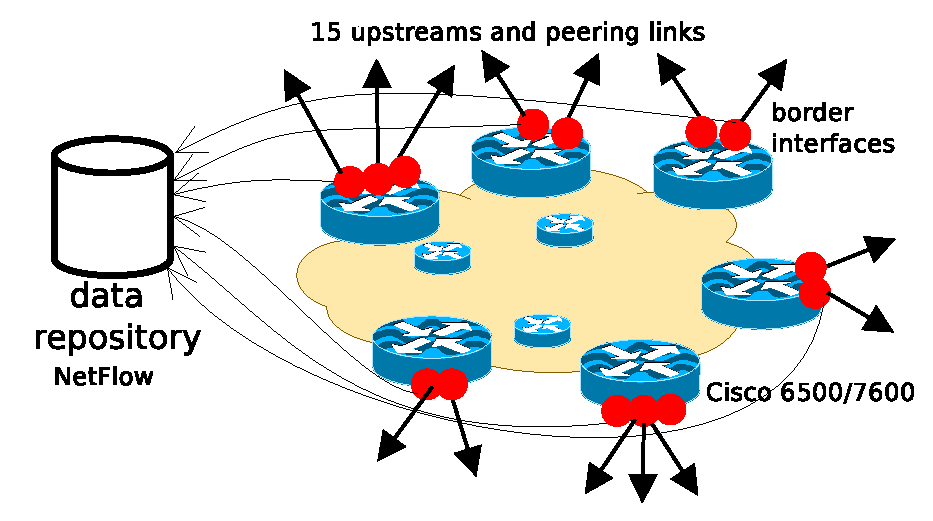
\includegraphics[width=12cm]{images/network_overview.eps}
	\caption{Overview of the SWITCH network \citep{SchatzmanThesis2012}} 
	\label{fig:switch_nework}
\end{figure}

Figure \ref{fig:switch_nework} provides an overview of the SWITCH network. 
Currently, SWITCH has 15 upstreams and peering links and is capturing flow level 
data at all external interfaces of their border routers by 2003 in form of 
unsampled \gls{netflow} data -- from 2003-2008 in version 5 and in version 9 
after 2008\citep{Schatzmann:Tracing}.

High traffic peak rates of more than 80'000 flows per second, 3 million packets 
per second and more than 20Gbit/s require hardware-based flow collection 
cards\citep{Schatzmann:Tracing}. \gls{TCP} flags are not available in the 
flow-level information because of limitations of the used hardware 
components\citep{Schatzmann:Tracing}. The generated flow data are collected and 
stored in a central data repository.

% briefly describe the Switch network and its topology..
% traffic volume and netflow data unsampled!
% see tech report 338 for numbers and layout?! evtl actual numbers (2012)
%%%%%%%%%%%%%%%%%%%%%%%%%%%%%%%%%%%%%%%%%%%%%%%%%%%%%%%%%%%%%%%%%%%%%%%%%%%%%%%%